% input files


% document's head
% \phantom{42}

\begin{center}
    \LARGE \textsc{Заметки курса <<Электричество и магнетизм>>}
\end{center}

\hrule

\phantom{42}

\begin{flushright}
    \begin{tabular}{rr}
    % written by:
        \textbf{Автор}: 
        & Хоружий Кирилл \\
        &\\
    % date:
        \textbf{От}: &
        \textit{\today}\\
    \end{tabular}
\end{flushright}

\thispagestyle{empty}
\tableofcontents
% \newpage



%%%%%%%%%%%%%%%%%%%%%%%%%%%%%%%%%%%%%%%%%%%%%%%%%%%%%%%%%%%%%%%%%%%%%%%%%%%%%%%%%%%
\secnum{1}{Криволинейные координаты и кинематика} % 1-6
%%%%%%%%%%%%%%%%%%%%%%%%%%%%%%%%%%%%%%%%%%%%%%%%%%%%%%%%%%%%%%%%%%%%%%%%%%%%%%%%%%%

\sbsnum{1}{Кинематика точки}
Для точки $P$ движущейся относительно некоторого неподвижного тела (свяжем с ним точку $O$), можно ввести следующие характеристики:
\begin{to_def}[Радиус вектор, скорость и ускорение точки $P$]
	\begin{equation*}
	\vc{r} = \overrightarrow{O P},
	\hspace*{1 cm}
	\vc{v} = \frac{d \vc{r}}{d \vc{t}},
	\hspace*{1 cm}
	\vc{w} =  \frac{d \vc{v}}{d t} = \frac{d^2 \vc{r}}{d t^2}.
\end{equation*}	
\end{to_def}

\begin{to_def}
	Для задания движения точки, зная её траекторию, можно сопоставить ей дуговую координату $\sigma (t)$ и получить выражения для скорости и ускорения, выраженные в осях \textit{естественного трёхгранника} $\vc{\tau}, \vc{n}, \vc{b}$.
	Таким образом для $\vc{r} = \vc{r}(\sigma(t))$:
	\begin{equation*}
		\vc{\tau} (\sigma) = \frac{d \vc{r}}{d \sigma}, 
		\hspace*{1 cm} 
		\frac{d \vc{\tau}}{d \sigma} = \frac{1}{\rho} \vc{n} (\sigma),
	\end{equation*}
	где $\rho$ -- радиус кривизны. Для кривой в $\mathbb{R}^3$ добавим ещё вектор $b$ для правой тройки. Таким образом получим формулы Френе:
	\begin{equation*}
		\frac{d \vc{\tau}}{d s} = \frac{1}{\rho} \vc{n},
		\hspace*{1 cm}
		\frac{d \vc{n}}{d s} = - \frac{1}{\rho} \vc{\tau} + \varkappa \vc{b},
		\hspace*{1 cm}
		\frac{d \vc{b}}{d s} = - \varkappa \vc{n}.
	\end{equation*}
\end{to_def}

Таким образом сможем в компонентах трёхгранника выписать скорость и ускорение точки:
\begin{gather*}
   \vc{v} = \frac{d \vc{r}}{d t} = \frac{d \vc{r}}{d \sigma} \frac{d \sigma}{d t} = v_\tau \vc{\tau}
   \\
   \vc{w} = \frac{d \vc{v}}{d t} = \frac{d_\tau}{d t} \vc{\tau} + v_\tau \frac{d \vc{\tau}}{d \sigma} \frac{d \sigma}{d t} = \frac{d^2 \sigma}{d t^2} \vc{\tau} + \frac{v_\tau^2}{\rho} \vc{n}.
\end{gather*}
Как видно, ускорение точки представилось в видео $w = w_n + w_\tau $ --- \textit{нормальной} и \textit{тангенциальной} составляющей.

\begin{to_lem}[Из матана]
	Для $f_i \in  C^2 \colon U \mapsto V$, если $X$ -- касательный вектор в точке $p \in U$, то $X(f)$ можно определить как:
	\begin{equation*}
		X(f) = X(x^i) \frac{\partial f(p)}{\partial x^i}, \text{ а координаты этого вектора в криволинейных координатах: } X = X^i \frac{\partial}{\partial x^i}.
	\end{equation*}
\end{to_lem}

Каждую материальную точку можем определить $\vc{r}_1, \ldots, \vc{r}_N$ -- итого $\mathbb{R}^{3N}$. Но есть некоторые ограничения вида
\begin{equation*}
    f_i (\vc{r}, t) = 0.
\end{equation*}
Вложим в фазовое пространство многообразие $M$, в котором локально всё хорошо. Тогда
$\dim M = n$ -- число степеней свободы, а параметризация $q_1, \ldots, q_N$ -- криволинейные координаты. В каждой $A \in M$ верно, что $\dot{\vc{q}} \in TM_A$, то есть
\begin{equation*}
    TM = \bigcup_q T_qM \ni (q, \dot{q})
\end{equation*}

И так, движение точки можно задать, если её криволинейные координаты --- известне функции $q(t)$.
\begin{equation*}
	\vc{r} = \vc{r}(q_1, q_2, q_3) = x \vc{i} + y \vc{j} + z \vc{k}.
\end{equation*}

\begin{to_def}
	\textit{Коэффициентами Ламе} такие $H^i$. C их помощью удобно выразить единичные базисные векторы криволинейных координат: 
	\begin{equation*}
		H_i = \left|\frac{\partial \vc{r}}{\partial q^i} \right| = \sqrt{\left(\frac{\partial x}{\partial q^i}\right)^2 + \left(\frac{\partial y}{\partial q^i}\right)^2 + \left(\frac{\partial z}{\partial q^i}\right)^2}.
		\hspace*{1 cm}
		e^i = \frac{1}{H_i} \frac{\partial \vc{r}}{\partial q^i}.
	\end{equation*}
\end{to_def}

Далее будем координатными векторами называть $\vc{g}_i(\vc{r}) = \frac{\partial \vc{r}}{\partial q^i}$. Разложение произвольного вектора по локальному базису имеет вид:
\begin{equation*}
	\vc{a} = a^i \vc{g}_i = a_j \vc{g}^j.
\end{equation*}
Здесь $\vc{g}^j$ --- векторы двойственного базиса к базису из $\vc{g}_i$. В двойственном же (взаимном) базисе из матана мы видели:
\begin{equation*}
	X(f) = d f (X) = \partial_x f,
	\hspace*{1 cm}
	d x^i (\frac{\partial}{\partial x^j}) = \frac{\partial x^i}{\partial x^j} = \delta_j^i,
	\hspace*{1 cm}
	a = a_i d x^i.
\end{equation*}
Таким образом получаем скорость точки и её ковариантную компоненту:
\begin{equation*}
	\vc{v} = \frac{d \vc{r}}{d t} = \frac{\partial \vc{r}}{\partial q^i} \frac{d q^i}{d t} = \vc{g}_i \dot{q}^i,
	\hspace*{1 cm}
	v^i = \vc{q}^i.
\end{equation*}
И для ускорения:
\begin{equation*}
	w_k = \left(\frac{d \vc{v}}{d t}\right)_k = \frac{(d \vc{v})_k}{d t} = g_{k j} \frac{d v^j}{d t} + \Gamma_{k i j} v^j v^i.
\end{equation*}


\sbsnum{2}{Описание движения твёрдого тела}
\begin{proof}[\ref{lem_6.20}]
	
	1) для введённой $\varphi$ достаточно: $\varphi_\varepsilon (x_1,\ldots,x_n) = A \varphi\left(\frac{\sqrt{n} x_1}{\varepsilon}\right)\ldots\varphi\left(\frac{\sqrt{n} x_n}{\varepsilon}\right)$.

	2) $\psi(x) = B \int_{-\infty}^x \varphi(t) \d t $, выбирем $B$: $\psi(x) \equiv 0 \; \forall x \leq 1$ и $\psi(x) \equiv 1 \; \forall x \geq -1$;

	3) достаточно положить: $\psi_{\varepsilon,\delta} (x) = \psi \left(\frac{\delta +\varepsilon -2|x|}{\varepsilon-\delta}\right)$.
\end{proof}

\sbsnum{3}{Приложения к твердому телу}
\begin{proof}[\ref{thr_6.21}]
	
	1) $f_k(x) - f(x) = \int_{\mathbb{R}^n} (f(x-t) - f(x)) \varphi_k(t) \d t$;

	2) Пусть $f$ р-но непр. в $U_\delta(K\subset \mathbb{R}^n) $ и пусть $|f(x) - f(y)|<\varepsilon$ при $|x-y|<\delta$ там же;

	3) Выбирая $k\colon 1/k <\delta$, тогда $\varphi_k(t) \neq 0 $ при $|t|<\delta$ и тогда $|f(x-t) - f(x)|<\varepsilon$ при $x \in K$.

	4) при $x \in K$ верна р-ная сходимость: $|f_k(x) - f(x)| \leq \varepsilon \int_{\mathbb{R}^n}\varphi_k(x) \d x = \varepsilon$.

	5) продифференцируем по параметру $\int_{\mathbb{R}^n} f(t) \varphi_k (x-t)\d t $;

	6) производная (5) при $x \in K$ будет зависеть только значений $f$ в $U_{1/k}(K)$, то есть $f$ можно считать интегрируемой при дифференцировании по параметру, что позволяет применять теорему.
\end{proof}

\begin{proof}[\ref{thr_6.22}]
	 По различным $\partial_{x_i} f*\varphi_k(x)$ получим по лемме \ref{lem_6.19}, для производных свёрток схожее равенство, с самой $f$, а значит и р-ную сходимость.
	\begin{equation*}
		\frac{\partial^m (f*\varphi_k)}{\partial x_{i_1}\ldots \partial x_{i_m}} = \frac{\partial^m f}{\partial x_{i_1}\ldots \partial x_{i_m}}*\varphi_k.
	\end{equation*}
\end{proof}

\begin{proof}[\ref{thr_6.23}]
	1) по thr(\ref{thr_5.75}) $f = h + g$, где $g$ -- эл. ступ., $\int_{\mathbb{R}^n} |h|\d x <\varepsilon$;

	2) по thr(\ref{thr_6.18}): $\int_{\mathbb{R}^n}|h * \varphi_k|\d x < \varepsilon$. То есть, если окажется: $\int_{\mathbb{R}^n}|g - g*`f_k|\d x < \varepsilon$, то
	\begin{equation*}
		\int_{\mathbb{R}^n}|f - f*\varphi_k| \d x \leq \int_{\mathbb{R}^n} |g - g* \varphi_k|\d x + \int_{\mathbb{R}^n}|h|\d x + \int_{\mathbb{R}^n} |h*\varphi_k| \d x < 3 \varepsilon.
	\end{equation*}

	3) Раскладывая $g$ в сумму х-их $\chi_P$, останется доказать для одной $\chi_P$;

	4) $\chi_P - \chi_P - \varphi_k \neq 0$ только в $U_{1/k}(\partial P) $ и по модулю $\leq 1$;

	5) То есть после интегрирования получим не более $\mu(U_{1/k}(\partial P))$.

	6) Напрямую можно убедиться, что эта $\mu \mapsto 0$ при $k\mapsto 0$.
\end{proof}

\sbsnum{4}{Сложное движение точки}
\subsubsection*{Теорема о сложении скоростей}
\begin{to_thr}
	Абсолютная скорость точки равна сумме переносной и относительной скорости: $\vc{v}^a = \vc{v}^e + \vc{v}^r$.
\end{to_thr}
\begin{proof}[$\triangle$]
	Для точки $P$ в абсолютной системе координат:
	\begin{equation*}
		\vc{R} = \vc{R}_0 + \vc{r}
		\hspace*{1 cm}
		\Rightarrow
		\hspace*{1 cm}
		\vc{v}_a = \vc{\dot{R}} = \vc{\dot{R}}_0 + \vc{\dot{r}} = \underbrace{\vc{v}_0 + \vc{\omega}\times \vc{r}}_{v^e} + \underbrace{A \vc{\dot{\rho}}}_{v^r}.
	\end{equation*}
	\textit{Переносная скорость} $v^e$ --- есть скорость той точки подвижной системы координат, в которой находится $P$.
	Таким образом показали напрямую разложение.
\end{proof}

\subsubsection*{Теорема Кориолиса}
\begin{to_thr}
	Абсолютное ускорение точки равно сумме переносного, относительного и карелысого ускорения: $w^a = w^e + w^r + w^c$.
\end{to_thr}
\begin{proof}[$\triangle$]
	Для абсолютного ускорения точки, продифференцируем ещё раз:
	\begin{equation*}
		\vc{w}^a = \vc{\dot{v}}_0 + \vc{\dot{\omega}} \times \vc{\dot{r}} + \vc{\omega} \times \vc{\dot{r}} + \dot{A} \vc{\dot{\rho}} + A \vc{\ddot{\rho}} = w_0 + \vc{\varepsilon} \times \vc{r} + \vc{\omega} \times (\vc{\omega} \times \vc{r} + A \vc{\dot{\rho}}) + \dot{A} \vc{\dot{\rho}} + A \vc{\ddot{\rho}}.
	\end{equation*}
	$\vc{\varepsilon}$ --- угловое ускорение подвижной системы координат, а $A \ddot{\rho} = w^r$:
	\begin{equation*}
		w^a = \underbrace{ w_0 + \vc{\varepsilon} \times \vc{r} + \vc{\omega} \times (\vc{\omega} \times \vc{r})}_{w^e} + w^r + \omega \times A \vc{\dot{\rho}} + \dot{A} \vc{\dot{\rho}}.
	\end{equation*}
	И последние два слогаемых дадут кареолисового ускорение: $\dot{A} \vc{\dot{\rho}} = \dot{A} A^{-1} A \vc{\dot{\rho}} = \vc{\omega} \times A \vc{\dot{\rho}} $, тогда получаем $w^c = 2 \vc{\omega} \times v^r$. Итого получаем искомую формулу.
\end{proof}


\sbsnum{5}{Вращение твёрдого тела}
% 6.4. Непрерывно дифференцируемые отображения и криволинейные системы координат

\begin{to_def} 
    \textit{Криволинейная замена координат} --- бесконечно гладкое отображение $\varphi \colon U \to V$ такое, что $\varphi^{-1}$ определено и тоже бесконечно гладко. 
\end{to_def}

\begin{to_lem} 
    Пусть открытое множество $U \subset \mathbb{R}^n $ выпукло. Для непрерывно дифференцируемого отображения $\varphi \colon U \to \mathbb{R}^m $ найдётся непрерывное отображение $A \colon U \times U \to \mathcal L (\mathbb{R}^n, \mathbb{R}^m)$, такое что $\forall x', \ x'' \in U$ 
\begin{equation*}
     \varphi(x'') - \varphi(x') = A(x', x'')(x'' - x')
 \end{equation*} 
 и $A(x, x) = D \varphi_x$.  
\end{to_lem}

% \begin{to_lem} 
%     Для всякого линейного отображения $A \colon \mathbb{R}^n \mapsto \mathbb{R}^m$ найдётся число $\|A\|$ такое что для все $x \in \mathbb{R}^n$ $|Ax| \leq \|A\| \cdot |x|$. 
% \end{to_lem}

\begin{to_thr}[Теорема об обратном отображении]
     \textbf{Если} отображение $\varphi \colon U \mapsto \mathbb{R}^n$ непрерывно дифференцируемо в окрестности точки $x$ \textbf{и} его дифференциал $D\varphi_x$ являетсяя невырожденным линейным преобразованием, \textbf{то} это отображение взаимно однозначно отображает некоторую окрестность $V \ni x$ на окрестность $W \ni y$, где $y = \varphi(x)$. Обратное отображение $\varphi^{-1} \colon W \to V$ тоже непрерывно дифференцируемо. 
\end{to_thr}


\begin{to_def} 
    \textit{Криволинейной системой координат} в окрестности точки $p \in \mathbb{R}^n$ называется набор таких функций, которые явяются координатами гладкого отображения окрестности $p$ на некоторое открытое множество в $\mathbb{R}^n$ с гладким обратным\footnote{
        По теореме об обратном отображении для проверки системы преобразования достаточно проверить невырожденность $\left(
    \partial y_i / \partial x_j
    \right)$ в точке $p$, или линейную независимость $dy^i$ в точке $p$.
    } отображением.
\end{to_def}



\sbsnum{6}{Общий случай движения твёрдого тела}
\begin{to_thr}[Теорема о неявной функции]
\label{thr_6.32}
     Пусть функции $f_1, \ldots, f_k$ непрерывно дифференцируемы в окрестности $p \in \mathbb{R}^n$ и 
    \begin{equation*}
        \det \left(
            \frac{\partial f_i}{\partial x_j} 
        \right) \neq 0
    \end{equation*}
    в этой окрестности. Пусть $f_i(p) = y_i$, $i = 1, \ldots, k$. Тогда найдётся окрестность точки $p$ вида $U \times V$, $U \subset \mathbb{R}^k$, $V \subset \mathbb{R}^{n-k}$, такая что в этой окрестности множество решений системы уравнений
    \begin{equation*}
        \left\{\begin{aligned}
            f_1(x) &= y_1, \\
            &\ldots \\
            f_k(x) &= y_k,
        \end{aligned}\right.
    \end{equation*}
    совпадает с графиком непрерывно дифференцируемого отображения $\varphi \colon V \to U$, заданного в координатах как
    \begin{equation*}
        \left\{\begin{aligned}
            x_1 &= \varphi_1 (y_1, \ldots, y_k,\ x_{k+1}, \ldots, x_n),\\
            &\ldots\\
            x_k &= \varphi_k (y_1, \ldots, y_k,\ x_{k+1}, \ldots, x_n),
        \end{aligned}\right.
    \end{equation*}
    то есть отображения $\mathbb{R}^{n-k} \mapsto \mathbb{R}^k$.
\end{to_thr}


\sbsnum{7}{ (и №26) Связи и всё, что с ними связанно}
\subsubsection*{Свободные и несвободные системы. Связи.}

В общем случае связь запишем, как
$$
    f(\vc{r}_\nu, \vc{v}_\nu, t) \geq 0.
$$
В частности, при $f(\vc{r}_\nu, \vc{v}_\nu, t) = 0$, связь называет \textit{двухсторонней}, или \textit{удерживающей}. При неравенстве, соотвественно, связь \textit{односторонняя}, \textit{освобождающая}.
Связь вида $f(\vc{r}_\nu, t) = 0$ называется \textit{геометрической}, \textit{конечная}, \textit{голономная}. Связь вида $f(\vc{r}_\nu, \vc{v}_\nu, t) = 0$ называется \textit{дифференциальной}, или \textit{кинематической}. Иногда кинематическая связь может быть представлена как геометрическая, такая связь называется \textit{интегрируемой}. 

\begin{to_def} 
     Если на систему материальных точек не наложены дифференциальные неинтегрируемые связи, то она называется голономной. Если же среди связей, наложенных на систему есть дифференциальные неинтегрируемые связи, то система называется неголономной.
\end{to_def}

Хотелось бы построить некоторую общую теорию для случая, когда этих связей несколько. 
В частности пусть есть $r$ геометрических связей.
\begin{equation}
\label{eqs1}
    f_\alpha (\vc{r}, t) = 0, \hspace{0.5cm} (\alpha = 1, \ldots, r),
\end{equation}
И несколько дифференциальных линейных связей
\begin{equation}
\label{eqs2}
    \sum_{\nu=1}^N \vc{a}_{\beta \nu} (\vc{r}_1, \ldots, \vc{r}_N, t) \cdot \vc{v}_\nu + a_\beta  (\vc{r}_1, \ldots, \vc{r}_N, t) = 0,
    \hspace{0.5cm} (\beta = 1, \ldots, s)
\end{equation}
Стоит сказать, что число \textit{степеней} \textit{свободы} данной системы:
$$
    3N - r - s \geq 1.
$$

\begin{to_def} 
     Геометрические связи называются стационарными или склерономными, если $t$ не входит в их уравнения \eqref{eqs1}. Дифференциальные связи \eqref{eqs2} называются \textit{стационарными} или \textit{склерономными} если функции $\vc{a}_{\beta\nu}$ не зависят явно от $t$, а функции $a_\beta \equiv 0$. Система называется \textit{склерономной}, если она либо свободная, либо на нее наложены только стационарные связи. Система называется \textit{реономной}, если среди наложенных на нее связей есть хотя бы одна нестационарная.
\end{to_def}

\subsubsection*{Ограничения, налагаемые связями на положения, скорости, ускорения и перемещения точек системы.}

Пусть задан некоторый момент $t = t*$. Тогда \textit{возможными положениями} назовём $\vc{r}_\nu$ такие, что для них верно \eqref{eqs1}, \eqref{eqs2}. 

Какие возможны скорости?
\begin{equation}
    \label{eqs3}
    \sum_{\nu=1}^N \frac{\partial f_\alpha}{\partial \vc{r}_\nu} \cdot \vc{v}_\nu +   \frac{\partial f_\alpha}{\partial t} = 0, \hspace{0.5cm} (\alpha = 1, \ldots, r).
\end{equation}

Совокупность векторов $\vc{v}_\nu = \vc{v}_\nu^*$, удовлетворяющая линейным
уравнениям \eqref{eqs2} и \eqref{eqs3} в возможном для данного момента времени положении
системы, назовем возможными скоростями. 

Какие возможны ускорения?
\begin{align}
\label{eqs4}
    \eqref{eqs3}, \eqref{eqs2}
    \hspace{0.25cm} \overset{d / dt}{\Rightarrow} \hspace{0.25cm} 
    & \sum_{\nu=1}^N \frac{\partial f_\alpha}{\partial \vc{r}_\nu} \cdot \vc{\mathrm{w}}_\nu +
    \sum_{\nu, \mu=1}^N \frac{\partial^2 f_\alpha}{\partial \vc{r}_\nu \partial \vc{r}_\mu} \vc{v}_\mu \cdot \vc{v}_\nu + 2 \sum_{k=1}^N \frac{\partial^2 f_\alpha}{\partial t \partial \vc{r}_\nu} \vc{v}_\nu + \frac{\partial^2 f_\alpha}{\partial t^2}  = 0 
    \hspace{0.25cm} &\alpha \in [1, r]\\
\label{eqs5}
    & \sum_{\nu=1}^N \vc{a}_{\beta\nu} \cdot \vc{\mathrm{w}}_\nu + \sum_{\nu, \mu =1}^N \frac{\partial \vc{a}_{\beta\nu}}{\partial \vc{r}_\mu} \vc{v}_\mu \cdot \vc{v}_\nu + \sum_{\nu=1}^N \frac{\partial \vc{a}_{\beta\nu}}{\partial t} \cdot \vc{v}_\nu + \sum_{\nu=1}^N \frac{\partial a_\beta}{\partial \vc{r}_\nu} \cdot \vc{v}_\nu + \frac{\partial  a_\beta}{\partial t} = 0
     \hspace{0.25cm} &\beta \in [1, s]
\end{align}

Совокупность векторов $\vc{\mathrm{w}}_\nu =\vc{\mathrm{w}}_\nu^*$, удовлетворяющая линейным
уравнениям \eqref{eqs4} и \eqref{eqs5} в возможном для данного момента времени положении
системы (+скорости), назовем возможными скоростями. 

Рассмотрим возможные перемещения $\Delta \vc{r}_\nu$ системы за $\Delta t$ из её возможного положения $\vc{r}_\nu^*$ в момент $t=t^*$. Тогда 
\begin{equation}
    \Delta \vc{r}_\nu = \vc{v}^* \Delta t + \frac{1}{2} \vc{\mathrm{w}}_\nu^* (\Delta t)^2 + \ldots
    \hspace{0.5cm} (\nu = 1, \ldots, N).
\end{equation}
Пренебрегая нелинейными членами, получим, что $\Delta \vc{r}_\nu = \vc{v}_\nu^* \Delta t$. Тогда, домножив \eqref{eqs2}, \eqref{eqs3} на $\Delta t$, получим систему уравнений, которой удовлетворяют линейные по $\Delta t$ возможные перемещения:
\begin{align}
\label{eqs7}
    \sum_{\nu=1}^N \frac{\partial f_\alpha}{\partial \vc{r}_\nu} \cdot \Delta \vc{r}_\nu + \frac{\partial f_\alpha}{\partial t} \Delta t &= 0,
    \hspace{0.5cm} &(\alpha = 1, \ldots, r), \\
\label{eqs8}
    \sum_{\nu=1}^N \vc{a}_{\beta\nu} \cdot \Delta \vc{r}_\nu + a_\beta \Delta t &= 0,
    \hspace{0.5cm} &(\beta = 1, \ldots, s),
\end{align}
где функции $\vc{a}_{\beta\nu}, a_\beta$ и частные производные вычисляются при $t=t^*, \; \vc{r}_\nu = \vc{r}_\nu^*$.


\subsubsection*{Действительные и виртуальные перемещения}
Пусть задано положение системы для $t, \vc{r}, \vc{v}, \vc{\mathrm{w}}$. Тогда для $t = t^* + dt$ запишем, что
\begin{equation}
\label{eqs9}
    \vc{r}_\nu (t^* + dt) - \vc{r}_\nu (t^*) = \vc{v}_{\nu_0}^* \d t + \frac{1}{2} \vc{\mathrm{w}}^*_{\nu_0} (dt)^2 + \ldots,
\end{equation}
где $\vc{\mathrm{w}}_{\nu_0}^*$ -- ускорения точек системы при $t = t^*$. Величины \eqref{eqs9} -- \textit{действительные (истинные) перемещения} точек системы за время $dt$. Тогда получим систему уравнений, аналогичную \eqref{eqs7}, \eqref{eqs8}:
\begin{align}
\label{eqs10}
    \sum_{\nu=1}^N \frac{\partial f_\alpha}{\partial \vc{r}_\nu} \cdot d \vc{r}_\nu + \frac{\partial f_\alpha}{\partial t} d t &= 0,
    \hspace{0.5cm} &(\alpha = 1, \ldots, r), \\
\label{eqs11}
    \sum_{\nu=1}^N \vc{a}_{\beta\nu} \cdot d \vc{r}_\nu + a_\beta d t &= 0,
    \hspace{0.5cm} &(\beta = 1, \ldots, s).
\end{align}


Помимо действительных перемещений есть \textit{виртуальные}. Ими называется совокупность величин $\delta \vc{r}_\nu$, удовлетворяющая линейным однородным уравнениям
\begin{align}
\label{eqs12}
    \sum_{\nu=1}^N \frac{\partial f_\alpha}{\partial \vc{r}_\nu} \cdot \delta \vc{r}_\nu  &= 0,
    \hspace{0.5cm} &(\alpha = 1, \ldots, r), \\
\label{eqs13}
    \sum_{\nu=1}^N \vc{a}_{\beta\nu} \cdot \delta \vc{r}_\nu  &= 0,
    \hspace{0.5cm} &(\beta = 1, \ldots, s),
\end{align}
Если система склерономна, то действительное перемещение будет одним из виртуальных.

\begin{to_def} 
    \textit{Синхронное варьирование} -- переход из одного положения в другое, при фиксированном времени
    $$
        \vc{r}_\nu^* \to \vc{r}_\nu^* + \delta \vc{r}_\nu.
    $$
    При синхронном варьировании мы не рассматриваем процесс движения и сравниваем допускаемые связями
    бесконечно близкие положения (конфигурации) системы для данного фиксированного момента времени.
\end{to_def}

Рассмотрим две совокупности возможных перемещений с одним и тем же значением величины $\Delta t$. Согласно разложению по Тейлору,
\begin{align*}
    \Delta_1 \vc{r}_\nu = \vc{v}_{\nu_1}^* \Delta t + \frac{1}{2} \vc{\mathrm{w}}_{\nu_1}^* (\Delta t)^2 + \ldots, \\
    \Delta_2 \vc{r}_\nu = \vc{v}_{\nu_2}^* \Delta t + \frac{1}{2} \vc{\mathrm{w}}_{\nu_2}^* (\Delta t)^2 + \ldots, 
\end{align*}
и рассмотрим их разность
$$
        \Delta_1 \vc{r}_\nu - \Delta_2 \vc{r}_\nu = (\vc{v}_{\nu_1}^* \Delta t - \vc{v}_{\nu_2}^* \Delta t) + \left(\frac{1}{2} \vc{\mathrm{w}}_{\nu_1}^* (\Delta t)^2 - \frac{1}{2} \vc{\mathrm{w}}_{\nu_2}^* (\Delta t)^2\right) + \ldots.
$$

\subsubsection*{Идеальные связи}
\begin{to_def}
	Связи называют \textit{идеальными}, если сумма работ этих связей на любых виртуальных перемещениях всегда равна нулю: $\sum \vc{R}_\nu \delta \vc{r}_\nu = 0$.
\end{to_def}

Абсолютно твердое тело является системой материальных точек, в которой на любые две точки наложена идеальная связь. При отсутствии других других связей, кроме между точками тела, твердое тело называют \textit{свободным}.

Считая связи идеальными запишем уравнения для материальных точек системы:
\begin{equation*}
	m_{\nu} \vc{w}_\nu = \vc{F}_\nu + \vc{R}_\nu
	\hspace*{0.3 cm}
	\Rightarrow
	\hspace*{0.3 cm}
	\left(
	\sum_{\nu=1}^N \vc{R}_\nu \delta \vc{r}_\nu = 0\right)
	\hspace*{0.3 cm}
	\Rightarrow
	\hspace*{0.3 cm}
	\sum_{\nu = 1}^{N}(\vc{F}_\nu - m_\nu \vc{w}_\nu) \delta \vc{r}_{\nu} = 0.
\end{equation*}
Последнее равенство называется общим уравнением динамики. Оно выполняется всегда для любого совместимого со связям движения, соответствующего заданным активным силам $\vc{F}{\nu}$.

Если же наоборот, дано какое-то совместимое со связями движение системы, для которого выполняется общее уравнение динамики, тогда с $\vc{R}_\nu = m_\nu \vc{w}_\nu - \vc{F}_\nu$ будем иметь равенства для задания уравнений несвободной системы. Мы считаем, что эти силы реакции реализуются в действительности и что рассматриваемое движение соответствует активным силам $\vc{F}_\nu (t,r_\nu, v_\nu)$.

Таким образом  \textit{общее уравнение динамики выражает необходимое и достаточное условие того, чтобы движение, совместимое со связями, соответствовало заданной системе активных сил}.

Взяв выражения для виртуальных перемещений всегда можно получить силы реакции так называемым методом \textit{множителей Лагранжа}:
\begin{equation*}
	\sum_{\nu=1}^N \left(\vc{R}_\nu - \sum_{i = 1}^d \lambda_i \frac{\partial f_i}{\partial \vc{r}_\nu} - \sum_{j = 1}^s \mu_j \alpha_{j \nu}\right) \delta \vc{r}_\nu = 0
	\hspace*{1 cm}
	\Rightarrow
	\hspace*{1 cm}
	\vc{R}_\nu = \sum_{i = 1}^d \lambda_i \frac{\partial f_i}{\partial \vc{r}_\nu} + \sum_{j = 1}^s \mu_j \alpha_{j \nu}.
\end{equation*}
Полученные выражения для реакций идеальных сил через неопределенные множители Лагранжа $\lambda_i $ и $\mu_j $ можно подставить в исходное уравнение связей, получим \textit{уравнения Лагранжа первого рода}:
\begin{equation*}
	m_\nu \vc{w}_\nu = \vc{F}_\nu + \sum_{i = 1}^d \lambda_i \frac{\partial f_i}{\partial \vc{r}_\nu} + \sum_{j = 1}^s \mu_j \alpha_{j \nu}.
\end{equation*}


%%%%%%%%%%%%%%%%%%%%%%%%%%%%%%%%%%%%%%%%%%%%%%%%%%%%%%%%%%%%%%%%%%%%%%%%%%%%%%%%%%%
% \secnum{2}{Основные теоремы динамики} % 9-13
%%%%%%%%%%%%%%%%%%%%%%%%%%%%%%%%%%%%%%%%%%%%%%%%%%%%%%%%%%%%%%%%%%%%%%%%%%%%%%%%%%%



%%%%%%%%%%%%%%%%%%%%%%%%%%%%%%%%%%%%%%%%%%%%%%%%%%%%%%%%%%%%%%%%%%%%%%%%%%%%%%%%%%%
% \secnum{3}{Уравнения движения твёрдого тела} % 14-18
%%%%%%%%%%%%%%%%%%%%%%%%%%%%%%%%%%%%%%%%%%%%%%%%%%%%%%%%%%%%%%%%%%%%%%%%%%%%%%%%%%%



%%%%%%%%%%%%%%%%%%%%%%%%%%%%%%%%%%%%%%%%%%%%%%%%%%%%%%%%%%%%%%%%%%%%%%%%%%%%%%%%%%%
\secnum{4}{Движение точки в центральном поле сил} % 19-21
%%%%%%%%%%%%%%%%%%%%%%%%%%%%%%%%%%%%%%%%%%%%%%%%%%%%%%%%%%%%%%%%%%%%%%%%%%%%%%%%%%%

\sbsnum{19}{Формулы Бине}
\begin{equation*}
    \alpha + \frac{\alpha}{\beta} 
\end{equation*}


%%%%%%%%%%%%%%%%%%%%%%%%%%%%%%%%%%%%%%%%%%%%%%%%%%%%%%%%%%%%%%%%%%%%%%%%%%%%%%%%%%%
\secnum{5}{Элементы механики сплошных сред} % 22-25
%%%%%%%%%%%%%%%%%%%%%%%%%%%%%%%%%%%%%%%%%%%%%%%%%%%%%%%%%%%%%%%%%%%%%%%%%%%%%%%%%%%

\sbsnum{22}{Сплошная среда и её напряжение}

\begin{to_lem}[Поведение интеграла формы при линейной замене координат]
     Интеграл дифференциальной формы $\nu \in \Omega_{\text{c}}^n (\mathbb{R}^n)$ при отображении $A^*$, соответствующем линейному преобразованию $A : \mathbb{R}^n \mapsto  \mathbb{R}^n$ меняет или не меняет знак в зависимости от знака определителя $\det A$, то есть
     \begin{equation*}
         \int_{\mathbb{R}^n} A^* \nu = (\sign \det A) \int_{\mathbb{R}^n} \nu.
     \end{equation*}
\end{to_lem}


\sbsnum{23}{Перемещение сплошной среды}
Пусть каждой точке среды соответсвует $\xi^1, \xi^2, \xi^3$, собственно $(\xi, t)$ -- \textit{лгранжевы переменные}. \textit{Закон движения среды} в таком случае это
\begin{equation}
    \vc{r} (\xi, t),
\end{equation}
скорость же
$$
    \vc{v} = \frac{\partial \vc{r}(\xi, t)}{\partial t},
    \hspace{0.5cm} 
    \vc{\mathrm{w}} = \frac{\partial \vc{v} (\xi, t)}{\partial t},
$$
и так далее.

Альтернативно можеем задать $(x, t)$ -- эйлерово описание. Тогда
$$
    \vc{v}(x, t), \vc{\mathrm{w}}(x, t) 
    \hspace{0.5cm} \text{-- поля скоростей и ускорений.}
$$

В частности, представляя движение по шоссе, полоса 1,2,3 и участок трассы -- эйлерово описание среды.
Если же мы будем следить за каждой машиной, то это будет лагранжево описание.

\sbsnum{24}{Тензоры деформаций и перемещений}
Длинная линия — модель линии передачи, продольный размер (длина) которой превышает длину волны, распространяющейся в ней. Такая линия передачи может быть охаракетризована погонными параметрами:
$R_0$ -- погонное сопротивление, $G_0$ -- паразитная, погонная проводимость, $L_0$ -- погонная индуктивность, $C_0$ -- погонная емкость.


Рассмотрим два рядом идущих длинных провода (коаксиальный кабель, например). Тогда в $z$ и $z+ \Delta z$ ток будет различным, как и, соответсвенно, разность потенцаилов. 
\begin{equation*}
    V(z+\Delta z) - V(z) = \frac{L_0 \Delta z}{c^2} \frac{\partial I}{\partial t},
    \hspace{1cm} 
    I(z) = I(z+\Delta z) + \frac{\partial q}{\partial t},
    \hspace{1cm} 
    q = C_0 \Delta z V.
\end{equation*}

\begin{figure}[h]
    \centering
    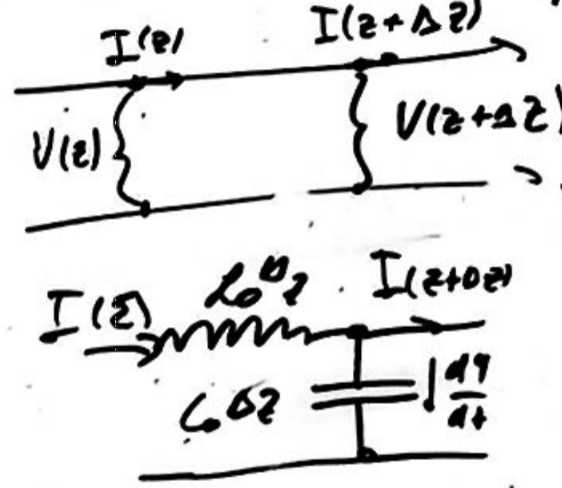
\includegraphics[width=0.25\textwidth]{img/2.png}
    %\caption{}
    %\label{fig:}
\end{figure}

\noindent
Из этих уравнений легко получить, что
\begin{equation}
    \left\{\begin{aligned}
        \frac{\partial U}{\partial z} &= - \frac{L_0}{c^2} \frac{d I}{d t} \\
        \frac{\partial I}{\partial z} &= - C_0 \frac{\partial U}{\partial t} 
    \end{aligned}\right.
    \hspace{0.5cm} \Rightarrow \hspace{0.5cm} 
    \boxed{
        \frac{\partial^2 U}{\partial t^2}  = \frac{c^2}{L_0 C_0} - \frac{\partial^2 V}{\partial z^2} 
    }.
\end{equation}
Решение аналогично будем искать в виде
\begin{equation}
    V = f_1 (z - vt) + f_2 (z + vt),
    \hspace{0.5cm} \Rightarrow \hspace{0.5cm} 
    v = \frac{c}{\sqrt{L_0 C_0}}.
\end{equation}
Кстати, если это всё посчитать для коаксиального кабеля, то
\begin{equation*}
    L_0 = 2 \mu \ln \frac{R_2}{R_1} , \hspace{0.5cm} 
    C_0 = \frac{\varepsilon}{2 \ln \frac{R_2}{R_1} },
    \hspace{0.5cm} \Rightarrow \hspace{0.5cm} 
    v = \frac{c}{\sqrt{\mu \varepsilon}}.
\end{equation*}


\subsubsection*{Коэффициент стоячей волны (standing wave ratio)}
Коэффициент стоячей волны -- отношение наибольшего значения амплитуды напряжённости электрического или магнитного поля стоячей волны в пучностях линии передачи к амплитуде в узлах.
КСВ является мерой согласования нагрузки (например, антенны) с линией передачи.

Наибольшее и наименьшее значения амплитуды соответсвенно равны
\begin{equation*}
    A_{\text{max}} = A_{\text{inc}} + A_{\text{ref}}, \hspace{0.5cm} 
    A_{\text{min}} = A_{\text{inc}} - A_{\text{ref}},
    \hspace{0.5cm} \Rightarrow \hspace{0.5cm} 
    \text{КСВ} = \frac{A_{\text{inc}} + A_{\text{ref}}}{A_{\text{inc}} - A_{\text{ref}}} = 
    \frac{1 + |\Gamma|}{1 - |\Gamma|},
\end{equation*}
где $|\Gamma|$ -- коэффициент отражения.

\subsubsection*{Согласованная нагрузка}
Рассмотрим длинную линию, пусть в цепи 
\begin{equation*}
    U = U_0 \cos \left(\omega_0 t - kz\right),  \hspace{0.5cm} 
    I = I_0 \cos \left(\omega_0 t - kz\right).
\end{equation*}
Сделаем следующий трюк. Возьмем, и продолжим линию до бесконечности, от которой, очевидно, ничего не отразится. Соотвественно нас интересует поиск эквивалентного импеданса системы. 
\begin{align*}
    U^* = U_0 \exp\left(i(\omega_0 t - kz)\right) &= U_0 e^{ikz} e^{-i\omega_0 t}, \\
    I^* = I_0 \exp\left(i(\omega_0 t - kz)\right) &= I_0 e^{ikz} e^{-i\omega_0 t}.
\end{align*}
Подставив эти выражения в волновое уравнение, и получим
\begin{equation*}
    ik U^* = i \omega_0 I^*,
    \hspace{0.5cm} 
    Z^* = U^* / I^* = \frac{\omega_0}{k},
    \hspace{0.5cm} \Rightarrow \hspace{0.5cm} 
    R = \frac{1}{c} \sqrt{\frac{L_0}{C_0}},
    \text{\ \ --- \ \ \textit{согласованная нагрузка}}.
\end{equation*}
То есть при наличии такого сопротивления на конце линии не будет никакого отражения. 




\sbsnum{25}{Элементы гидродинамики}
\subsubsection*{Уравнение непрерывности}
\begin{to_def}[Предмет рассмотрения]
	Ввиду макроскопического рассмотрения \textit{жидкости}(газы) в гидродинамике представлется как сплошная среда, то есть малый элемент объёма жидкости содержит ещё достаточно больше количество молекул, относительно межмолекулярного расстояния.
\end{to_def}

Для описания движения жидкости требуется задать распределение скорости жидкости $\vc{v} = \vc{v}(x,y,z,t)$ и какие-либо её две термодинамические величины, как, например, плотность и давление. Важно отметить, что все эти величины относятся не к отдельной частице, а к точке в пространстве в определенное время.

\begin{to_thr}[Уравнение непрерывности]
\phantom{239}

\begin{proof}[$\triangle$]
	В маленьком объёме $V_{0}$ количество жидкости есть $\int_{V_0} \rho d V$.
	Через элемент поверхности, ограничивающей $V_0$, в единицу времени протекает $\rho \vc{v} \cdot d \vc{f}$ жидкости --- положительно или отрицательное число, в зависимости от того, вытекает или втекает жидкость соответственно.
	Тогда приравниваем для вытекания жидкости два наших рассуждения:
	\begin{equation*}
		- \frac{\partial}{\partial t} \int \rho d V =  \oint \rho \vc{v} \cdot d \vc{f}
		\hspace*{0.5 cm} 
		\Rightarrow 
		\hspace*{0.5 cm}
		\int \left(\frac{\partial \rho}{\partial t} + \div \rho \vc{v}\right)d V = 0
		\hspace*{0.5 cm}
		\Rightarrow
		\hspace*{0.5 cm}
		\frac{\partial \rho}{\partial t} + \div \rho \vc{v} = 0.
	\end{equation*}
	Последнее следует из того, что равенство должно иметь для любого объёма, таким образом получили искомое \textit{уравнение непрерывности}.
\end{proof}
	
\end{to_thr}

\subsubsection*{Уравнение Эйлера}

\begin{to_thr}[Уравнение Эйлера]
\phantom{239}

\begin{proof}[$\triangle$]
	Выделим в жидкости некоторый объём, полная сила, действующая на этот объём: $- \oint p d \vc{f} = - \int \grad p d V$, где интеграл из взятого по поверхности объёма преобразуется в сам рассматриваемый объём.
	Таким образом получили, что на единицу объёма жидкости будет действовать сила:
	\begin{equation*}
		\rho \frac{d \vc{v}}{d t} = - \grad p.
	\end{equation*}
	Однако стоящая здесь скорость определяет изменение скорости именно элемента объёма, а не точки в пространстве.
	Запишем это изменение скорости:
	\begin{equation*}
		d \vc{v} 
		=
		 \frac{\partial \vc{v}}{\partial t} d t + \frac{\partial \vc{v}}{\partial x^i} d x^i 
		= 
		\frac{\partial \vc{v}}{\partial t} d t + (d \vc{r} \cdot \nabla) \vc{v}
		\hspace*{1 cm}
		\Rightarrow
		\hspace*{1 cm}
		\frac{\partial \vc{v}}{\partial t} + (\vc{v} \nabla) \vc{v} = - \frac{1}{\rho} \grad p.
	\end{equation*}
	Последнее и есть искомое уравнение Эйлера.
\end{proof}
\end{to_thr}

Если же жидкость движется во внешнем поле тяжести, то, на каждый элемент объёма будет действовать сила, которая просто добавится к изначальному уравнению: 
\begin{equation*}
	\frac{\partial \vc{v}}{\partial t} + (\vc{v} \nabla) \vc{v} = - \frac{\nabla p}{\rho} + \vc{g}.
\end{equation*}

\subsubsection*{Уравнение Навье-Стокса}

Чтобы нормально учесть вязкость, нужно поговорить про \textit{поток импульса}.
Импульс единицы объёма жидкости есть $\rho \vc{v}$, скорость изменения его компоненты:
\begin{equation*}
	\frac{\partial}{\partial t} \rho v^i = \rho \frac{\partial v^i}{\partial t} + \frac{\partial \rho}{\partial t} v^i.
\end{equation*}
Уравнения непрерывности и Эйлера запишутся в тензорном виде:
\begin{equation*}
	\frac{\partial \rho}{\partial t} = - \frac{\partial (\rho v^k)}{\partial x^k},
	\hspace*{0.5 cm}
	\hspace*{0.5 cm}
	\frac{\partial v^i}{\partial t} = - v^k \frac{\partial v^i}{\partial x^k} - \frac{1}{\rho} \delta^{i k} \frac{\partial p}{\partial x^k}.
\end{equation*}
Тогда получим:
\begin{equation*}
	\frac{\partial}{\partial t} \rho v^i 
	= 
	- \rho v^k \frac{\partial v^i}{\partial x^k} -  \delta^{i k} \frac{\partial p}{\partial x^k} - v^i \frac{\partial \rho v^k}{\partial x^k} 
	=
	-\delta^{i k} \frac{\partial p}{\partial x^k} - \frac{\partial}{\partial x^k} \rho v^i v^k
	= - \frac{\partial \Pi^{i k}}{\partial x^k}.
\end{equation*}
\begin{to_def}
	$\Pi^{i k} $ --- \textit{тензор плотности потока импульса}:
	$
		\Pi^{i k} = p \delta^{i k} + \rho v^i v^k.
	$
\end{to_def}

Таким образом уравнение Эйлера у нас записалось в виде:
$
	\frac{\partial}{\partial t} \rho v^i = - \frac{\partial \Pi^{i k}}{\partial x^k}.
$
Поток импульса представляет собой чисто обратимый перенос импульса, связанный с просто механическим передвижением различных участков жидкости и с действующими в жидкости силами давления.
\textit{Вязкость} (внутреннее трение) жидкости проявляется в наличии ещё дополнительного, необратимого переноса импульса из мест с большой скоростью в места с меньшей.

Поэтому уравнение движения вязкой жидкости можно получить, прибавив к идеальному потоку импульса дополнительный член $\sigma^{i k}_{visc}$, определяющий такой вязкий перенос:
$
\Pi^{i k} = p \delta^{i k} + \rho v^i v^k - \sigma^{i k}_{visc} = - \sigma^{i k} + \rho v^i v^k.
$
\begin{to_def}
	Таким образом: $\sigma^{i k} = - p \delta^{i k} + \sigma^{i k}_{visc}$ называют \textit{тензором напряжений}, а $\sigma^{i k}_{visc}$ --- вязким тензором напряжений.
\end{to_def}

Чтобы написать выражение для вязкого напряжения сделаем пару оговорок. 
\textit{Во первых}, градиенты скорости движения участков жидкости относительно друг друга не велики, тогда $\sigma^{i k}_{visc}$ зависит лишь от первых производных скорости по координатам, линейно. \textit{Во вторых}, не зависящие от первых производных величины должны обращаться в нуль как для скорости потока $\vc{v} = \const$ и тензор должен быть нулевым. \textit{В третьих}, $\sigma^{i k}_{visc} = 0$ когда жидкость совершает целое равномерное вращение, поскольку никакого внутреннего трения тогда не будет.
Для такого равномерного вращения с $\vc{v} = [\vc{\omega} \vc{r}]$ линейными комбинациями производных обращающимися в нуль будут: $\frac{\partial v^i}{\partial x^k} + \frac{\partial v^k}{\partial x^i}$.

Это всё даёт нам мотивацию для не шибко сильных потоков несжимаемой жидкости согласится с Сэром Исааком Ньютоном, и написать тензор вязкого напряжения, как \textit{тензор скорости деформации}:
\begin{equation*}
	\sigma^{i k}_{visc} = \eta \left(\frac{\partial v^i}{\partial x^k} + \frac{\partial v^k}{\partial x^i}\right),
	\hspace*{1 cm}
	\Rightarrow
	\hspace*{1 cm}
	\sigma^{i k} = - p \delta^{i k} + \eta \left(\frac{\partial v^i}{\partial x^k} + \frac{\partial v^k}{\partial x^i}\right).
\end{equation*}
А уравнение Эйлера тогда для несжимаемой жидкости запишется:
\begin{equation*}
	\rho \left(\frac{\partial v^i}{\partial t} + v^k \frac{\partial v^i}{\partial x^k}\right)
	=
	- \delta^{i k} \frac{\partial p}{\partial x^k} + \frac{\partial}{\partial x^k} \left[\eta \left(\frac{\partial v^i}{\partial x^k} + \frac{\partial v^k}{\partial x^i}\right)\right].
\end{equation*}
а в более человеческом, привычном глазу, виде \textit{уравнение Навье-Стокса для несжимаемой жидкости}:
\begin{equation*}
	\frac{\partial \vc{v}}{\partial t} + (\vc{v} \triangle) \vc{v} = - \frac{1}{\rho} \grad p + \frac{\eta}{\rho} \Delta \vc{v}.
\end{equation*}
\begin{to_def}
	Коэффициент $\eta$ называется --- \textit{динамическим коэффициентом вязкости}, а отношение $\eta/\rho = \nu$ --- \textit{кинематической вязкостью}.
\end{to_def}



%%%%%%%%%%%%%%%%%%%%%%%%%%%%%%%%%%%%%%%%%%%%%%%%%%%%%%%%%%%%%%%%%%%%%%%%%%%%%%%%%%%
\secnum{6}{Принципиальность виртуальных перемещений} % 26-30
%%%%%%%%%%%%%%%%%%%%%%%%%%%%%%%%%%%%%%%%%%%%%%%%%%%%%%%%%%%%%%%%%%%%%%%%%%%%%%%%%%%

\sbsnum{27}{Общее уравнение динамики (принцип Даламбера-Лагранжа)}
Пусть $\vc{r}_\nu = \vc{r}_\nu (t), \ \vc{v}_\nu = \dot{\vc{r}}_\nu(t)$, тогда для их истинности необходимо и достаточно
\begin{equation*}
    \sum_{\nu=1}^N \left(
        \vc{F}_\nu - m_\nu \vc{\mathrm{w}}_\nu
    \right) \cdot \delta \vc{r}_\nu = 0.
\end{equation*}


\begin{proof}[$\triangle$]
    Пусть $\vc{r}_\nu$ отвечает истинным движениеям, тогда $\vc{F}_\nu - m_\nu \vc{\mathrm{w}}_\nu = - \vc{R}_\nu$, тогда томножив на $\vc{r}_\nu$ -- получили доказательство достаточности.
    Докажем необходимость. Пусть $m_\nu \vc{\mathrm{w}}_\nu - \vc{F}_\nu = \vc{\Phi}_\nu$, тогда $\sum \vc{\Phi}_\nu \cdot \delta \vc{r}_\nu = 0$. Тогда 
    \begin{equation*}
        \vc{\Phi}_\nu = \sum_{\alpha=1}^r \gamma_\alpha \frac{\partial f}{\partial \vc{r}_\nu} 
        + \sum_{\beta=1}^s \lambda_\beta \vc{a}_{\beta \nu}.
    \end{equation*}
    Подставив, получим уравнения Лагранжа, так что всё хорошо.
\end{proof}
































\sbsnum{28}{(вплоть до №30) Общее уравнение динамики, статики и т.д.}

Легко получить соотношение вида
\begin{equation}
    \sum_{i=1}^N \left(
        \vc{F}_i - m_i \vc{\mathrm{w}}_i
    \right) \cdot \delta \vc{r}_i = 0.
\end{equation}
Данное соотношение является необходимым и достаточным условием для того, чтобы движение, совместимое с идеальными связями, отвечало данной системе активных сил $\vc{F}_i$. Оно получило название \textbf{общего уравнения динамики} или \textit{дифференциальным вариационным принципом Даламбера-Лагранжа}.

\begin{to_thr} [принцип Даламбера-Лагранжа]
Верно, что
\begin{equation*}
    m_i \vc{\mathrm{w}}_i = \vc{F}_i + \vc{R}_i,
    \hspace{0.5cm} \Rightarrow \hspace{0.5cm} 
    \sum_i \left(
       \vc{F}_i -  m_i \vc{\mathrm{w}}_i
    \right) \cdot \delta \vc{r}_i = 0.
\end{equation*}
\end{to_thr}

Аналогично можно сформулировать \textit{принцип Журдена}
\begin{equation}
    \sum_{i=1}^N \left(
        \vc{F}_i - m_q \vc{\mathrm{w}}_i
    \right) \cdot \vc{v}_i = 0,
\end{equation}
и \textit{принцип Гаусса}:
\begin{equation}
    \sum_{i=1}^N \left(
        \vc{F}_i - m_q \vc{\mathrm{w}}_i
    \right) \cdot \vc{v}_i = 0,
\end{equation}
где $\delta \vc{\mathrm{w}}_i = \vc{\mathrm{w}}^*_{i_1} - \vc{\mathrm{w}}^*_{i_2}$ не обязательно малая величина. 

Замечая, что $m_i = \const$, а $\vc{F}_i = \vc{F}_i (p, q)$, то последнее уравнение перепишется в виде
\begin{equation*}
    Z = \frac{1}{2} \sum_{i=1}^N m_i 
    \left(
        \vc{\mathrm{w}}_i - \frac{\vc{F}_i}{m_i} 
    \right)^2,
    \hspace{1cm} 
    \delta Z = 0,
\end{equation*}
где величина $Z$ называется принуждением или мерой принуждения. К слову она не просто стационарна для истинных движений. 

\texttt{Истинным является движение с минимальной мерой принуждения.} Другими словами \textit{несвободная система совершает движение, наиболее близкое к свободному}. 

\begin{to_def} 
    Будем считать, что $q^0 \in M$ -- \textit{точка равновесия}, если при $\dot{q}^0 \equiv \dot{q}(0) \equiv 0$ приводит к $q(t) = q^0$. 
\end{to_def}

В таком случае верен следующий принцип:

\begin{to_thr}[принцип Лагранжа]
    Для того, чтобы точка была положением равновесия на $t \in [t_1, t_2]$ необходимо и достаточно, чтобы сумма элементарных работ на $\forall$ виртуальных перемещениях всех активных сил была равна нулю.
    \begin{equation}
        \delta A \big|_0 = 0 
        \hspace{0.5cm} 
        \delta A = \sum_i \vc{F}_i \cdot \delta \vc{r}_i,
        \hspace{0.5cm} (t\in[t_1, t_2])
    \end{equation}
    что является \textbf{общим уравнением статики}.
\end{to_thr}

Этот принцип можно рассматривать, как дракона с тремя головами. Вот если система \textbf{голономная}, то
\begin{equation*}
    \delta A = Q_i \delta q_i 
    \hspace{0.5cm} \Rightarrow \hspace{0.5cm} 
    Q_i = 0 \ \forall i.
\end{equation*}
Если система \textbf{консервативная}, то
\begin{equation*}
    Q_1 = - \frac{\partial P}{\partial q^i} 
    \hspace{0.5cm} \Rightarrow \hspace{0.5cm} 
    \text{положение равновесия --- стационарная точка потенциала}.
\end{equation*}
Если же у нас \textbf{твёрдое тело}, тогда
\begin{equation*}
    \delta A = \left(
        \vc{R}^{\text{внеш}} \cdot \vc{v}_O
    \right) \d t + 
    \left(
        \vc{M}_O^{\text{внеш}} \cdot \vc{\omega}
    \right) dt
    \hspace{0.5cm} \Rightarrow \hspace{0.5cm} 
    \left\{\begin{aligned}
        \vc{R}^{\text{внеш}} &= 0 \\
        \vc{M}^{\text{внеш}} &= 0 \\
    \end{aligned}\right.
\end{equation*}




%%%%%%%%%%%%%%%%%%%%%%%%%%%%%%%%%%%%%%%%%%%%%%%%%%%%%%%%%%%%%%%%%%%%%%%%%%%%%%%%%%%
\secnum{7}{Уравнения Лагранжа} % 31-34
%%%%%%%%%%%%%%%%%%%%%%%%%%%%%%%%%%%%%%%%%%%%%%%%%%%%%%%%%%%%%%%%%%%%%%%%%%%%%%%%%%%

\sbsnum{31}{Уравнение Лагранжа второго рода}
\begin{to_lem}[Разбиение единицы в окрестности компакта на многообразии]
     Пусть $M$ -- гладкое многообразие, а $K \subseteq M$ -- его компактное подмножество. Для любого покрытия $\{U_\alpha\}_\alpha$ компакта $K$ открытыми множествами найдётся набор неотрицательных гладких функций $\{\rho_\alpha\}_\alpha$ с компактными носителями $\mathrm{supp}\, \rho_\alpha$ таких, что
\begin{equation*}
    \forall \alpha \ \textnormal{supp}\, \rho_\alpha \subset U_\alpha,
\end{equation*}
    только конечное число из них отлично от нуля и
    $\sum_\alpha \rho_\alpha (x) \equiv 1$
    в некоторой окрестности $K$.
\end{to_lem}

\begin{to_def} 
    Интеграл дифференциальной формы $\nu \in \Omega_{\text{c}}^n (M)$ с компактным носителем по ориентированному $n$-мерному многообразию $M$ определяется с помощью разбиения единицы в окрестности носителя $\nu$ 
    \begin{equation*}
         \rho_1 + \ldots + \rho_m = 1,
     \end{equation*} 
     подчиненного некоторому набору положительно ориентрированных карт как
     \begin{equation*}
         \int_M \nu = \sum_i \int_M \rho_i \nu_i,
     \end{equation*}
     где интегралы справа рассматриваются в координатных картах, содержащих носители соответствующих $\rho_i$.
\end{to_def}

\begin{to_lem} 
    Определение интеграла не зависит от выбора системы положительных карт в данной ориентации и подчиненного им разбиения единциы. 
\end{to_lem}





\sbsnum{32}{Разрешимость уравнений Лагранжа}
Подставим разложение кинетической энергии в уравнения Лагранжа, оставив только слагаемые с обобщёнными ускорениями $f_j (q, \dot{q}, t) = a_{jk} \ddot{q}^j$. 
\begin{equation*}
    T = \frac{1}{2} \sum_\nu m_\nu \dot{\vc{r}}_\nu^2 = \frac{1}{2} \sum_\nu
    \left(
        \frac{\partial \vc{r}_\nu}{\partial q^j} \dot{q}^j + \frac{\partial \vc{r}_\nu}{\partial t} 
    \right)^2 = 
    \frac{1}{2} 
    \bigg[
    \underbrace{
        a_{jk} \dot{q}^j \dot{q}^k
    }_{
        2T_2
    } +
    \underbrace{
        a_j \dot{q}^j
    }_{
        2T_1
    } +
    \underbrace{
        a_0
    }_{
        2T_0
    }
    \bigg],
\end{equation*}
где коэффициенты, соответственно, равны 
\begin{equation*}
    a_{jk}(q, t) = \sum_\nu m_\nu \frac{\partial \vc{r}_\nu}{\partial q^j} \cdot \frac{\partial \vc{r}_\nu}{\partial q^k},
    \hspace{0.5cm} 
    a_j(q, t) = \sum_\nu m_\nu \frac{\partial \vc{r}_\nu}{\partial q^j} \cdot \frac{\partial \vc{r}_\nu}{\partial t},
    \hspace{0.5cm} 
    a_0 = \sum_\nu m_\nu 
    \left(
    \frac{\partial \vc{r}_\nu}{\partial t} 
            \right)^2.
\end{equation*}
Для склерономных систем $\partial \vc{r}_\nu / \partial t = 0$, соотвественно $T = a_{jk} \dot{q}^j \dot{q}^k$, при чём $a_{jk} \equiv a_{jk} (q)$.

Теперь подставим значение $T$ в уравнения Лагранжа, и получим, что
$
    a_{ik} \ddot{q}^k = f_i,
$
где $f_1 = f_1(q, \dot{q}, t)$. Уравнений в системе $n$, причём $a_{jk}$ является положительно определенной формой\footnote{
    \red{Требует отдельного доказательства.}
}, соответственно невырожденной. 

\begin{to_thr} 
    Уравнения Лагранжа второго рода разрешимы относительно обобщенных ускорений 
\end{to_thr}


\sbsnum{37}{Ковариантность уравнений Лагранжа}
\begin{to_tas}
	Для не обязательно компактного многообразия без края $M$ рассмотрим дифференциальные формы с компактным носителем $\Omega_c^*(M)$ и определим когомологии де Рама с компактным носителем:
	\begin{equation*}
		H_c^k (M) = \left(ker d \colon \Omega_c^k (M) \rightarrow \Omega^{k+1}_c (M)\right) / \Im \d \colon \Omega_c^{k-1}(M) \rightarrow \Omega_c^{k}(M).
	\end{equation*}

	Если $ \dim M = n$, M ориентируемо и связно, \textbf{то} $H_c^n(M)$ одномерно.
\end{to_tas}

\begin{to_tas}
	$H_c^k (\mathbb{R}^n) = 0$ при $k \neq n$, и $H_c^n(\mathbb{R}^n) = \mathbb{R} $.
\end{to_tas}

\sbsnum{33}{Изменение полной мехнической энергии голономной системы}
Пусть есть также непотенциальные силы, часть обобщенных сил, соответстующих непотенциальным силам, обозначим $Q_i^*$, тогда
\begin{equation*}
    Q_1 = - \frac{\partial \Pi}{\partial q^i} + Q_i^*,
    \hspace{0.5cm} \Rightarrow \hspace{0.5cm} 
    \frac{d }{d t} \frac{\partial T}{\partial \dot{q}^i} - 
    \frac{\partial T}{\partial q^i} 
    =
    - \frac{\partial \Pi}{\partial q^i} + Q_i^*.
\end{equation*}
Найдём производную по времени от кинетической энергии
\begin{equation*}
    \frac{d T}{d t} = 
    \frac{\partial T}{\partial \dot{q}^i} \ddot{q}^i + \frac{\partial T}{\partial q^i} \dot{q}_i + \frac{\partial T}{\partial t}  =
    \frac{d }{d t} \left(
        \frac{\partial T}{\partial \dot{q}^i} \dot{q}^i
    \right) - \left(
        \frac{d }{d t} \frac{\partial T}{\partial \dot{q}^i} - \frac{\partial T}{\partial q^i} 
    \right) \dot{q}^i + \frac{\partial T}{\partial t}.
\end{equation*}
По \textit{теореме Эйлера об однороных функциях} для $f(x_1, \ldots, x_n)$ $k$-й степени верно что
\begin{equation*}
    \frac{\partial f}{\partial x^i} x^i = kf,
    \hspace{0.5cm} \Rightarrow \hspace{0.5cm} 
    \frac{\partial T}{\partial \dot{q}^i} \dot{q}^i = 2 T_2 + T_1.
\end{equation*}
В таком случае последнее равеноство перепишется, как
\begin{align*}
    \frac{d T}{d t} 
    &=
    \frac{d }{d t} (2 T_2 + T_1) + \frac{\partial \Pi}{\partial q^i} \dot{q}^i - Q_i^* \dot{q}^i + \frac{\partial T}{\partial t} 
    = \\ &= 
    \frac{d }{d t} (2 T_2 + 2 T_1 + 2 T_0) - \frac{d }{d t} (T_1 + 2 T_0) + \frac{d \Pi}{d t} - \frac{\partial \Pi}{\partial t} - Q_i^* \dot{q}^i + \frac{\partial T}{\partial t}.
\end{align*}
Таким образом мы доказали следующую теорему.

\begin{to_thr}
     Полная мехническая энергия голономной системы $E = T+ \Pi$ изменяется следующим образом:
     \begin{equation*}
         \frac{d E}{d t} = N^* + \frac{d }{d t} (T_1 + 2 T_0) + \frac{\partial \Pi}{\partial t} - \frac{\partial T}{\partial t}.
     \end{equation*}
     Где $N^* = Q_i^* \dot{q}^i$ -- мощность непотенциальных сил.
\end{to_thr}


\begin{to_def} 
    Голономная склерономная система с  $\Pi \equiv \Pi(q)$ называется \textit{консервативной}, при чём $d E / d t = 0$.
\end{to_def}

\subsubsection*{Гироскопические силы}


\begin{to_def} 
    Непотенициальные силы называют \textit{гироскопическими}, если их мощность равна $0$. 
\end{to_def}


Пусть $Q_i^* = \gamma_{ik} \dot{q}^k$. Если $\gamma_{ik} = -\gamma_{ki}$, то силы $Q_i^*$ гиросокопические, соответсвенно кососимметричность $\gamma_{ik}$ необходима и достаточна.

Более того, имеет место равеноство

\vspace{-25pt}
\begin{equation*}
    \sum_\nu \vc{F}_\nu \cdot \vc{v}_\nu = \sum_\nu \vc{F}_\nu \cdot
    \left(
        \frac{\partial \vc{r}_\nu}{\partial q^i} \dot{q}^i + \frac{\partial \vc{r}_\nu}{\partial t} 
    \right) 
    =
     \bigg(
     \overbrace{
     \sum_\nu \vc{F}_\nu \cdot \frac{\partial \vc{r}_\nu}{\partial q^i}
     }^{
     Q_i
     }
      \bigg)
     \dot{q}^i + \sum_\nu \vc{F}_\nu \cdot \frac{\partial \vc{r}_\nu}{\partial t},
     \hspace{0.25cm} \overset{\partial \vv{r}_\nu / \partial t = 0}{=}  \hspace{0.25cm} 
     \sum_\nu \vc{F}_\nu \cdot \vc{v}_\nu = Q_i \dot{q}^i.
\end{equation*}
Поэтому для склерономных систем $N^* = 0$ выражается в $\sum_\nu \vc{F}_\nu^* \cdot \vc{v}_\nu = 0$.

\subsubsection*{Диссипативные силы}

\begin{to_def} 
    Непотенциальные силы называются диссипативными, если их $N^* \leq 0$, но $N^* \not \equiv 0$. При $\Pi = \Pi(q)$ и диссипативности сил $d E / dt \leq 0$, тогда система называется диссипативной. В случае определенно-отрицательной $N^* (\dot{q})$ дисспация называется \textit{полной}, а в случае знакопостоянной отрицательной $N^*$ \textit{частичной}.
\end{to_def}

\begin{to_def} 
    \textit{Диссипативной функцией Рэлея} называется  положительная квадратичная форма $R$ такая, что
    \begin{equation*}
        R = \frac{1}{2} b_{ik} \dot{q}^i \dot{q}^k,
        \hspace{1cm}
        Q_i^* = - \frac{\partial R}{\partial \dot{q}^i}  = - b_{ik} \dot{q}^k.
    \end{equation*}
    Тогда для склерономной системы можность $N^*$ непотенциальных сил равна
    \begin{equation*}
        \sum_\nu \vc{F}_\nu^* \cdot \vc{v}_\nu = Q_i^* \dot{q}^i = - 2 R \leq 0.
    \end{equation*}
\end{to_def}






\sbsnum{34}{Обобщенный потенциал и первые интегралы лагранжевых систем}
Физический потенциал силового поля в математический терминах означает поиск $f \in C^\infty (M) \colon \d f = \alpha$ для заданной силы $\alpha \in \Omega^1(M)$

\begin{to_def} 
	Пусть $\vc{A}$ -- векторное поле в области $D \subset \mathbb{R}^n$. Функция $U \colon D \mapsto \mathbb{R}$ называется \textit{потенциалом поля} $\vc{A}$ в области $D$, если в этой области $\vc{A} = \grad U$. Поле, обладающее потенциалом, называется \textit{потенциальным полем}. 
\end{to_def}

\begin{to_thr}
	Необходимым и достаточным условием наличия потенциала у непрерывной $\alpha \in \Omega^1(M)$, для гладкого $M$, является независимость $\int_\gamma \alpha$ от выбора  кусочно-гладкой кривой $\gamma$ между двумя точками.

	Эквивалентно можно потребовать равенства нулю интегралов по всем замкнутым кусочно-гладким кривым.
	\label{thr_7.1}
\end{to_thr}

\begin{to_lem}[Необходимое условие потенциальности]
	 Необходимым условием существования потенциала у $\alpha \in \Omega^1(M)$ является $\d \alpha = 0$ (т.к. $\d (\d u) = 0$).
\end{to_lem}

\begin{to_lem} 
	В случае $\mathbb{R}^3$ по определению $d \omega^1_{\vv{A}} = \omega^2_{\rot \vv{A}}$, поэтому необходимое условие потенциальности поля $\vc{A}$ переписывается в виде $\rot \vc{A} = 0$.
\end{to_lem}

Однако этого не достаточно, так например в открытой $U = \mathbb{R}^2 \backslash \{ 0 \}$:
\begin{equation*}
	\alpha = \frac{x \d y - y \d x}{x^2 + y^2}
	\hspace*{0.5 cm} \leadsto \hspace*{0.5 cm}
	\d \alpha = 0,
	\hspace*{0.5 cm} \text{ но } \hspace*{0.5 cm}
	\oint_{S^1} \alpha = 2 \pi.
\end{equation*}


\begin{to_def} 
	Поле $\vc{A}$ называется \textit{векторным потенциалом} поля $\vc{B}$ в области $D \subset \mathbb{R}^3$, если в этой области выполняется соотношение $\vc{B} = \rot \vc{A}$. 
\end{to_def}

Это можно переписать в виде $\omega^2_{\vv{B}} = d \omega^1_{\vv{A}}$, тогда $\omega^3_{\div \vv{B}} = d \omega_{\vv{B}}^2 = d^2 \omega^1_{\vv{A}} = 0$, то есть необходимое условие $\div \vc{B} = 0$, принято такое поле называть \textit{соленоидальным}. 










%%%%%%%%%%%%%%%%%%%%%%%%%%%%%%%%%%%%%%%%%%%%%%%%%%%%%%%%%%%%%%%%%%%%%%%%%%%%%%%%%%%
\secnum{8}{Канонические уравнения} % 35-41 \ 38-39
%%%%%%%%%%%%%%%%%%%%%%%%%%%%%%%%%%%%%%%%%%%%%%%%%%%%%%%%%%%%%%%%%%%%%%%%%%%%%%%%%%%

\sbsnum{35}{Гамильтонов формализм, уравнения и интеграл Якоби}
\begin{to_def}
	Диф-форма $\alpha \in \Omega^k (M)$ --- замкнутая, если $\d \alpha = 0$; $\alpha$ --- точная, если $\exists \beta \in \Omega^{k-1} (M) \colon \d \beta = \alpha$.
	\label{def_7.9}
\end{to_def}

\begin{to_tas}
	Если $\alpha$ --- точная, а $\beta$ --- замкнутая, \textbf{то} $\alpha \wedge \beta$ --- точная.
	\label{tas_7.10}
\end{to_tas}

\begin{to_def}
	Отображения $h_0, h_1 \colon M \rightarrow N$ гладко гомотопны, если $\exists h \colon M \times [0,1] \rightarrow N$, такое что $h_0(x) = h(x,0)$ и $h_1(x) = h(x,1)$.
	\label{def_7.12}
\end{to_def}

Многообразие $M \times [0,1]$ (цилиндр) является топологическим пространством, которое локально устроено как произведение открытого $U\subset \mathbb{R}^n$ на отрезок.
Интересно заметить, что если $\partial M = \varnothing$, то $\partial(M \times [0,1]) = M \times {0,1}$. 

\begin{to_def}
	М называется стягиваемым в точку $x_0 \in M$ или гомотопным точке, если $\exists h \colon M \times [0,1] \rightarrow M$ такое, что $h(x,1) = x$ и $h(x,0) = x_0$. ($\mathbb{R}^n$ --- $h(x,t) = t x$)
\end{to_def}

\begin{to_thr}[Теорема Пуанкаре]
	$\forall \omega \in \Omega^{k+1}(M)$, замкнутая на стягиваемом в точку $M$, является точной.
	\label{thr_poin}
\end{to_thr}

В умных книжках говорят чаще про непрерывные гомотопии, но так как мы работаем с гладкими $M$, мы будем использовать гладкие гомотопии. Обладая определенной сноровкой можно показать, что если два отображения между многообразиями непрерывно гомотопны, то они и гладко гомотопны.

Станет легче, если свести вопрос к случаю, когда для $\varepsilon > 0$: $h(x,t) = h(x,0)$ при $t < \varepsilon$ и $h(x,t) = h(x,1)$ при $t > 1-\varepsilon$.
Определим новую гомотопию:
\begin{equation*}
\varphi(\in C^\infty) \colon \mathbb{R} \rightarrow [0,1]:
\left\{
\begin{aligned}
	&\varphi = 0,\; t \leq \varepsilon\\
	&\varphi = 1,\; t \geq 1-\varepsilon
\end{aligned}
\right.
\hspace*{0.5 cm}  \leadsto \hspace*{0.5 cm}
	h'(x,t)=h(x,\varphi(t)).
\end{equation*} 

\begin{to_thr}[Цепная гомотопия]
	Если отображения $f_0, f_1 \colon M \rightarrow N$ гладко гомотопны, \textbf{то} $\forall \alpha \in \Omega^k (N)$ выполняется для некоторой $H \colon \Omega^k (N) \rightarrow \Omega^{k-1}(M)$:
	\begin{equation*}
		f_1^* \alpha - f_0^*\alpha - H(\delta \alpha) + \delta(H(\alpha)).
	\end{equation*}
\end{to_thr}

\sbsnum{36}{Принцип наименьшего действия}
\subsubsection*{Пара слов от Александра Вадимовича}


\begin{to_def} 
    \textit{Действием по Гамильтону} называют функционал вида
    \begin{equation*}
         S = \int_{t_0}^{t_1} L(\gamma(t), \dot{\gamma}(t), t) \d t.
    \end{equation*} 
    Переходя к однопараметрическому семейству кривых $\gamma(\alpha, t)$ получим \textit{вариацию действия}
    \begin{equation*}
        S = \int_{t_0}^{t_1} L(\gamma(\alpha, t), \dot{\gamma}(\alpha, t), t) \d t, 
        \hspace{0.5cm} 
        \delta S = \frac{d S}{d \alpha} \delta \alpha.
    \end{equation*}
\end{to_def}


\begin{to_thr}[принцип Гамильтона]
    Кривая $\gamma(\alpha, t)$ является экстремалью действия тогда и только тогда, когда является решением уравнений Лагранжа
     \begin{equation*}
         \delta S = 0
         \hspace{0.5cm} \Leftrightarrow \hspace{0.5cm} 
         \gamma(\alpha, t) \in \textnormal{Sol}\,
         \left(
     \frac{d}{dt} \frac{\partial L}{\partial \dot{q}^k} - \frac{\partial L}{\partial q^k} = 0
         \right)
         .
     \end{equation*}
\end{to_thr}


\begin{proof}[$\triangle$]
    Давайте просто проварьируем Лагранжиан, тогда
    \begin{align*}
        \delta S 
        &=
         \int_{t_0}^{t_1} 
        \left(
            \frac{\partial L}{\partial q^i} \frac{\partial q^i}{\partial \alpha} +
            \frac{\partial L}{\partial \dot{q}^i} \frac{\partial \dot{q}^i}{\partial \alpha}  
        \right) \delta \alpha \d t 
        =
        \int_{t_0}^{t_1} \left(
            \frac{\partial L}{\partial q^i} \delta q^i + \frac{\partial L}{\partial \dot{q}^i} \delta \dot{q}^i
        \right) \d t
        =
        \frac{\partial L}{\partial \dot{q}} \partial q \bigg|_{t_1}^{t_2}
        + \int_{t_1}^{t_2}
        \left(
            \frac{\partial L}{\partial q^i} - \frac{d }{d t} \frac{\partial L}{\partial \dot{q}^i} 
        \right) \,\delta q^i \d t
        = 0.
    \end{align*}
    таким образом уравнения Лагранжа выполнены. 
\end{proof}


\subsubsection*{Истинные и окольные пути}

\begin{to_def} 
    Совокупность траекторий, которые описаны перемещениями из начальных положений $a_\nu$ в конечные $b_\nu$, образуют \textit{истинный} (\textit{действительный, прямой}) путь системы $\gamma_\nu$.

    Совокупность $\gamma_\nu'$, бесконечно близких к $\gamma_\nu$ и таких, что движение точки по кривой $\gamma_\nu'$ может происходить без нарушения связей, называют окольным путем системы.
\end{to_def}

\begin{to_def} 
    \textit{Расширенное координатным пространство} помимо криволинейных координат $q^i$ также время $t$.
\end{to_def}

\begin{to_def} 
    При достаточном удалении точки $A_1$ от точки $A_0$ может оказаться, что краевая задача имеет решения, соответствующие бесконечно близким прямым путям в расширенном координатном пространстве. В этом случае точки $A_0$ и $A_1$ называют \textit{сопряженными кинетическими фокусами}. 
\end{to_def}

\begin{to_lem} 
    Положение точки на окольном пути задается, как $\vc{r}_\nu (t) + \delta \vc{r}_\nu(t)$, где $\delta \vc{r}_\nu (t_0) = 0$ и $\delta \vc{r}_\nu (t_1) = 0$. Синхронное варьирование и взятие производной по времени перестановочны. 
\end{to_lem}

\subsubsection*{Принцип Гамильтона-Остроградского}

Рассмотрим прямой путь и совокупность окольных путей. Пусть $m_\nu$ -- масса точки $P_\nu$, а $\vc{F}_\nu$ -- равнодействующая \textit{активных}\footnote{
    \red{Определение бы написать.}
} сил, приложенных к точке. Тогда
\begin{equation*}
    \int_{t_0}^{t_1} \sum_{\nu=1}^{N} \vc{F}_\nu \cdot \delta \vc{r}_\nu \d t - 
    \sum_{\nu=1}^N m_\nu \int_{t_0}^{t_1} \vc{\mathrm{w}}_\nu \cdot \delta \vc{r}_\nu \d t = 0.
\end{equation*}
Рассмотрим разность между значениями $T(t)$ на окольном и прямом путях
\begin{equation*}
    \delta T = \frac{1}{2} \sum_{\nu=1}^N m_\nu \left(
        \dot{\vc{r}}_\nu + \delta \dot{\vc{r}}_\nu
    \right)^2 - \frac{1}{2} \sum_{\nu=1}^N m_\nu \dot{\vc{r}}_\nu^2 = 
    \sum_{\nu=1}^N m_\nu \dot{\vc{r}}_\nu \cdot \delta \dot{\vc{r}}_\nu,
\end{equation*} 
таким образом
\begin{equation*}
     \int_{t_0}^{t_1} \delta T \d t = \sum_{\nu=1}^N  m_\nu \int_{t_0}^{t_1} \dot{\vc{r}}_\nu \cdot d \delta \vc{r}_\nu = \sum_{\nu=1}^N m_\nu \dot{\vc{r}}_\nu \cdot \delta \vc{r}_\nu 
    \bigg|_{t_0}^{t_1} - \sum_{\nu=1}^N m_\nu \int_{t_0}^{t_1} \vc{\mathrm{w}}_\nu \cdot \delta \vc{r}_\nu \d t = 
    - \sum_{\nu=1}^N  m_\nu \int_{t_0}^{t_1} \vc{\mathrm{w}}_\nu \cdot \partial \vc{r}_\nu \d t.
\end{equation*}
Таким образом мы пришли к следующей теореме:

\begin{to_thr}[принцип Гамильтона-Остроградского]
     Если величины $\delta \vc{r}_\nu (t)$ соответствуют синхронному варьированию прямого пути и $\delta \vc{r}_\nu (t_0) = \delta \vc{r}_\nu (t_1) = 0$ тогда и только тогда, когда
     \begin{equation*}
         \int_{t_0}^{t_1} \left(
            \delta T + \sum_{\nu=1}^N \vc{F}_\nu \cdot \delta \vc{r}_\nu
         \right) \d t = 0.
     \end{equation*}
\end{to_thr}

\begin{proof}[$\triangle$]
    Хотелось бы также показать, что из принципа Гамильтона-Остроградского вытекает уравнения Лагранжа второго рода:
\begin{equation*}
    \left\{\begin{aligned}
        \sum_{\nu=1}^N \vc{F}_\nu \cdot \delta \vc{r}_\nu = Q_i \delta q^i \\
        \delta T = \frac{\partial T}{\partial q^i} \delta q^i + \frac{\partial T}{\partial \dot{q}^i} \delta \dot{q}^i
    \end{aligned}\right.
    \hspace{0.5cm} \Rightarrow \hspace{0.5cm} 
    \int_{t_0}^{t_1} \sum_{\nu=1}^N 
    \left[
        \frac{\partial T}{\partial \dot{q}^i} \delta \dot{q}^i + \left(
            \frac{\partial T}{\partial q^i} + Q_i
        \right) \delta q^i
    \right] \d t = 0.
\end{equation*}
Интегрируя по частям находим, что
\begin{equation*}
    \int_{t_0}^{t_1} \frac{\partial T}{\partial \dot{q}^i} \delta \dot{q}^i \d t 
    = 
    \int_{t_0}^{t_1} \frac{\partial T}{\partial \dot{q}^i} d \delta q^i 
    = 
    \frac{\partial }{\partial \dot{q}^i} \delta q^i \bigg|_{t_0}^{t_1} 
    - \int_{t_0}^{t_1} \frac{d }{d t} \frac{\partial T}{\partial \dot{q}^i} \delta q^i \d t 
    = 
    - \int_{t_0}^{t_1} \frac{d }{d t} \frac{\partial T}{\partial \dot{q}^i} \delta q^i \d t.
\end{equation*}
Таким образом приходим к равенству вида
\begin{equation*}
    \int_{t_0}^{t_1} \left(
        \frac{d }{d t} \frac{\partial T}{\partial \dot{q}^i} - \frac{\partial T}{\partial q^i} - Q_i
    \right) \delta q^i \d t = 0,
    \hspace{0.5cm} \Rightarrow \hspace{0.5cm} 
    \frac{d }{d t} \frac{\partial T}{\partial \dot{q}^i} - \frac{\partial T}{\partial q^k} = Q_k.
\end{equation*}
Следовательно принцип Гамильтона-Остроградского может быть положен в основу динамики голономных систем.
\end{proof}



\subsubsection*{Принцип Гамильтона-Остроградского для систем в потенциальном поле сил}

В потенциальном поле сил верно, что
\begin{equation*}
    \sum_{\nu=1}^N \vc{F}_\nu \cdot \delta \vc{r}_\nu = - \delta \Pi,
    \hspace{0.5cm} \Rightarrow \hspace{0.5cm} 
    \int_{t_0}^{t_1} (\delta T - \delta \Pi) \d t = 0,
    \hspace{0.5cm} \overset{L = T - \Pi}{\Rightarrow}  \hspace{0.5cm} 
    \int_{t_0}^{t_1} \delta L \d t = 0.
\end{equation*}

\begin{to_def} 
    \textit{Действием по Гамильтону} для голономных систем называется интеграл вида
    \begin{equation*}
        S = \int_{t_0}^{t_1} L \d t.
    \end{equation*}
\end{to_def}

\begin{to_thr}[Принцип Гамильтона-Остроградского v2]
     Для голономной системы в случае существования потенциала сил среди всех путей выделяется прямой путь тем, что для него $\delta S = 0$.
\end{to_thr}



\subsubsection*{Экстремальное свойство действия по Гамильтону}
\begin{to_thr}[принцип наименьшего действия]
    В окрестности, достаточно малой, чтобы отсутствовали кинетические фокусы, действие по Гамильтону на прямом пути будет наименьшим, по сравнению с окольными, проходимыми за то же время.
\end{to_thr}


\begin{proof}[$\triangle$]
    Пусть $[af]$ и $[ac]$ действие на двух различных путях системы. Для их разности имеем
    \begin{equation*}
        [ac]-[af]
        =
        \int_{t_0}^{t_1} \sum_{\nu=1}^N \left(
            m_\nu \vc{v}_\nu \cdot \delta \dot{\vc{r}}_\nu - \frac{\partial \Pi}{\partial \vc{r}_\nu} \cdot \delta \vc{r}_\nu
        \right) \d t 
        =
        \sum_{\nu=1}^N  m_\nu \vc{v}_\nu (t) \cdot \delta \vc{r}_\nu (t) 
        + 
        \int_{t_0}^{t_1} \sum_{\nu=1}^N (\vc{F}_\nu - m_\nu \vc{\mathrm{w}}_\nu) \cdot \delta \vc{r}_\nu \d t.
    \end{equation*}
    где $\vc{v}_\nu$ и $\partial |pi / \partial \vc{r}_\nu$ вычисляются по $a_\nu f_\nu$.
    Учитывая общее уравнение динамики, это соотношение можно переписать в виде
    \begin{equation*}
        [ac]-[af] = \sum_{\nu=1}^N m_\nu v_\nu(f) \cos \alpha_\nu \delta s_\nu,
    \end{equation*}
    где $\alpha_\nu$ -- угол между $v_\nu$ и $\delta \vc{r}_\nu$, а $\delta s_\nu$ -- длина $f_\nu c_\nu$.
    \red{Опуская некоторые выкладки,} можем теперь получить, что $S_{\text{ок}} > S_{\text{пр}}$.
\end{proof} 





\sbsnum{40}{Принцип Мюпертюи-Лагранжа}
\red{Хорошо бы посмотреть на происходящее ещё с точки зрения Льва Давидовича, как в задаче о движение луча.}
\begin{to_def} 
    Рассмотрим голономную (обобщенно) консервативную систему. Рассмотрим движение в $n$-мерном координатном пространстве. Рассмотрим прямые и окольные пути такие, что $H = h = \const$. При таком \textit{изоэнергетическом варьировании} $t_1-t_0$ не обязательно одинаково для прямого и окольного пути.     
\end{to_def}

\subsubsection*{Принцип Мопертюи-Лагранжа}

\begin{to_def} 
    При заданной $h$ уравнения движения могут быть записаны в форме Якоби, они также будут иметь форму уравнений Лагранжа, где $L \to P$, $t \to q_1$. По аналогии с действием $S$ по Гамильтону введём \textit{действие по Лагранжу}:
\begin{equation*}
    W = \int_{q_0^1}^{q_1^1} P \d q^1.
\end{equation*} 
\end{to_def}


\begin{to_thr}[Принцип Мопертюи-Лагранжа\footnote{
    Или \textit{принцип наименьшего действия Якоби}.
}]
     Среди всех кинематически возможных путей голономной консервативной системы, прямой путь выделяется тем, что для него действие по Лагранжу $W$ имеет стационарное значение $\delta W = 0$.
\end{to_thr}

Аналогично экстремальное значение будет принимать действие по Лагранжу при отсутствие кинематических фокусов в рассматриваемой области. 

Как было показано раннее функция Якоби $P$ может быть вычислена, как
\begin{equation*}
    W = \int_{q_0^1}^{q_1^1} P \d q^1 = \int_{q_0^1}^{q_1^1} \frac{2T}{\dot{q}^1} \d q^1 = \int_{t_0}^{t_1} 2 T \d t.
\end{equation*}
Важно заметить, что $T + \Pi = \const$,  а вот $t_1$ не зафиксировано. Иначе можно переписать
\begin{equation*}
    W = \int_{t_0}^{t_1} \sum_{\nu=1}^N m_\nu v_\nu^2 \d t 
    =
    \sum_{\nu=1}^N \int_{s_\nu^0}^{s_\nu^1} m_\nu v_\nu \d s_\nu,
\end{equation*}
т.е. для консервативной системы действие по Лагранжу равно сумме работ количеств движения точек системы на соответствующих их перемещениях.

















\sbsnum{41}{Принцип Якоби и геодезические}
\red{Про геодезические можно написать больше и лучше.}
Рассмотрим консервативную энергию с $n$ степенями свободы. Кинетическая энергия -- $T = \frac{1}{2} a_{ik} \dot{q}^i \dot{q}^k$. Введём в координатном пространстве метрику
\begin{equation*}
    ds^2 = 2 T dt^2 = a_{ik} \d q^i \d q^k,
    \hspace{0.5cm} \Rightarrow \hspace{0.5cm} 
    T = \frac{1}{2} \left(\frac{d s}{d t} \right)^2,
\end{equation*}
т. е. в такой метрике $T$ системы равная изображающей точки в координатном пространстве, если считать, что изображающая точка обладает массой, равной единице.

Если система движется по инерции, т.е. $\Pi = 0$, то из интеграла $T + \Pi = h = \const$ и тогда
\begin{equation*}
    \frac{d s}{d t} = \sqrt{2 h},
    \hspace{0.5cm} \Rightarrow \hspace{0.5cm} 
    W = 2 \int_{t_0}^{t_1} T \d t = 2 h (t_1 - t_0) = \sqrt{2h} l,
\end{equation*}
где $l = \sqrt{2h} (t_1-t_0)$ -- длина кривой, пройденной за время $t_1-t_0$. Из \textit{принцип Якоби} следует, что $\delta l = 0$, т.е. задача свелась к задаче дифгема о поиска геодезической.

Пусть теперь движение в потенциальном поле $(\Pi \neq 0)$. Тогда функция Якоби $P$:
\begin{equation*}
    W = \int_{q^{1}_1}^{q_1^1} P \d q^1 = 
    2 \int_{q^{1}_1}^{q_1^1}
    \sqrt{ (h - \Pi) G} \d q^1 
    =
    \sqrt{2} \int_{q^{1}_1}^{q_1^1} 
    \sqrt{
        (h-\Pi) a_{ik} \d q^i \d q^k
    }.
\end{equation*}
Область движения ограничена $\Pi \leq h$, так что введём новую метрику $d \sigma^2$, по формуле
\begin{equation*}
    d \sigma^2 = (h - \Pi) a_{ik} \d q^i \d q^k,
    \hspace{0.5cm} \Rightarrow \hspace{0.5cm} 
    W = \sqrt{2} \sigma,
\end{equation*}
где $\sigma$ -- длина дуги. Теперь нахождение траекторий снова свелось к нахождению геодезической!)

Далее рассмотрим две задачи, раскрывающих эту тему.













 
% \subsubsection*{Задача о траектории луча (оптический принципа Ферма $\sim$ принципа Мопертеи-Лагранжа)}

Найдём траекторию светового луча в среде с показателем преломления
\begin{equation*}
    n(z) = n_0 + n_z z.
\end{equation*}
Согласно принципу Ферма, введя $(ds)^2 = (dr)^2 + (dz)^2$, считая $dz / dr = \dot{z}$
\begin{equation*}
    \delta \left(
        \int_A^B (n_0 + n_z z) \d s
    \right) = 0,
\hspace{0.5cm} \Rightarrow \hspace{0.5cm} 
    \delta
    \left(
        \int_A^B z \sqrt{1 + \dot{z}^2} \d r
    + \frac{n_0}{n_z}  l 
    \right) = 0,
\end{equation*}
где
\begin{equation*}
    l = \int_A^B \sqrt{1 + \dot{z}^2} \d r.
\end{equation*}
Вспомнив \eqref{lstar} и \eqref{intl}, 
поймём, что решаем изопериметрическую задачу, которую уже решили в предыдущем пункте, решением является траектория по цепной линии, с $\lambda = -n_0/n_z$:
\begin{equation}
    z(r) = \frac{n_0}{n_z} + C_1 \ch \frac{r-C_2}{C_1},
\end{equation}
где $C_1$ и $C_2$ определяются из начальных условий\footnote{
    Предполагая, что мы хотим пустить луч от точки $(z_1, r_1)$ к $(z_2, r_2)$, мы сможем сделать это единственным образом, это и задаст $C_1$ и $C_2$.
}.



\subsubsection*{Задача о цепной линии}

Решим задачу о цепной линии. Пусть в точках $(x_1, y_1)$ и $(x_2, y_2)$ закреплена цепь с линейной плотностью $\rho$ и массой $M$.
Для цепной линии сначала найдём центр масс $y_0$:
\begin{equation*}
    y_0 = \frac{1}{M} \int_{x_1}^{x_2}
    y \cdot 
    \underbrace{
    \rho \sqrt{1 + (y_x')^2} \d x
    }_{
    dm
    }.
\end{equation*}
Лагранжиан системы
\begin{equation*}
    L = T - \Pi = M g \cdot y_0.
\end{equation*}
В силу независимости $L$ от $t$ верно, что
\begin{equation}
    \delta S = \delta 
    \left(\int_{t_1}^{t_2} L \d t\right)
    = 0,
    \hspace{0.5cm} \Rightarrow \hspace{0.5cm} 
    \delta L = 0, \hspace{0.5cm} \Rightarrow \hspace{0.5cm}
    \delta
    \bigg(
    \int_{x_1}^{x_2}
    \underbrace{
    y \sqrt{1 + (y_x')^2}
    }_{
    F(x)
    } \d x
    \bigg) = 0
    ,
\end{equation}
что позволяет нам решать немного другую задачу.

Мы знаем, что на $\dot{q}, q$ равносильны следующие условия
\begin{equation*}
    \frac{d }{d t} \frac{\partial L(\dot{q}, q, t)}{\partial q^i}  - \frac{\partial L}{\partial q}  = 0,
    \hspace{0.5cm} \Leftrightarrow \hspace{0.5cm} 
    \delta \left(
        \int_{t_1}^{t_2} L(\dot{q}, q, t) \d t
    \right) = 0,
\end{equation*}
при фиксированной длине нити $l$ равной
\begin{equation}
\label{intl}
    l = \int_{x_1}^{x_2} \underbrace{
    \sqrt{1+\dot{y}^2}
    }_{\varphi(x)} \d x,
\end{equation}
где $y_x' = \dot{y}$ (здесь и далее). 
Тогда введём\footnote{
    О причинах такого решения см. метод решения изопериметрической задачи.
} $L^*$
\begin{equation}
\label{lstar}
    L^* (y, x) = F(x) - \lambda \varphi(x),
\end{equation}
для которого верно, что
\begin{equation}
\label{maeq}
\delta \left(\int_{x_1}^{x_2} L^*(y, \dot{y}, x) \d x \right) = 0
\hspace{0.5cm} \Leftrightarrow \hspace{0.5cm} 
    \frac{d}{dx} \frac{\partial L^*}{\partial \dot{y}} -\frac{\partial L^*}{\partial x} = 0.
\end{equation}
Формально мы перещли к решению изопериметрической задачи. Для удобство переобозначим $L^* = L$. 
Посмотрим на $\partial L / \partial \dot{y} = L_{\dot{y}}$:
\begin{equation*}
    d L_{\dot{y}} (y, \dot{y}) = 
    \frac{\partial L_{\dot{y}}}{\partial y} \d y + 
    \frac{\partial L_{\dot{y}}}{\partial \dot{y}} \d \dot{y},
    \hspace{0.5cm} \Rightarrow \hspace{0.5cm} 
    \frac{d }{d x} \frac{\partial L}{\partial \dot{y}} -\frac{\partial L}{\partial y} =
    L_{\dot{y}, y} \dot{y} + L_{\dot{y}, \dot{y}} \ddot{y} - L_{y} = 0.
\end{equation*}
Домножив на $(-\dot{y})$ получим, как видно, полный дифференциал \rotatebox[origin=c]{270}{:)}
\begin{equation*}
    \frac{\partial L}{\partial y} \frac{d y}{d x} 
    + \underbrace{
    \frac{\partial L}{\partial \dot{y}} \frac{d \dot{y}}{d x} 
    - \bigg(
        \frac{\partial L}{\partial \dot{y}} \ddot{y}
    }_{\text{прибавил/вычел}}
     + 
        \dot{y} \bigg[
            \frac{\partial L_{\dot{y}}}{\partial y} \dot{y} + \frac{\partial L_{\dot{y}}}{\partial \dot{y}} \ddot{y}
        \bigg]
    \bigg)
    = \frac{d }{d x} \left(
        L - \dot{y} \frac{\partial L}{\partial \dot{y}} 
    \right),
\end{equation*}
откуда \eqref{maeq} может быть переписано, как
\begin{equation*}
    L - \dot{y} \frac{\partial L}{\partial \dot{y}} = C_1,
\end{equation*}
то есть да, <<энергия>> сохраняется, $x$ же явно не входит в $L^*$. 

Конкретно в нашем случае,
\begin{equation*}
    (y+\lambda) \sqrt{1 + \dot{y}^2}
    - \dot{y} (y + \lambda) \frac{\dot{y}}{\sqrt{1+\dot{y}^2}}  = C_1,
    \hspace{0.5cm} \Rightarrow \hspace{0.5cm} 
    y + \lambda = C_1 \sqrt{1 + \dot{y}^2}.
\end{equation*}
Как известно 
\href{https://ru.wikipedia.org/wiki/%D0%A8%D0%B8%D0%BD%D1%83%D1%81}{шинус} замечателен: $1 + \sh^2 \varkappa = \ch^2 \varkappa$, так что пусть $\dot{y} = \sh \varkappa$. Тогда
\begin{equation*}
    y = C_1 \ch \varkappa - \lambda.
\end{equation*}
Подставив друг в друга последних два выражения, найдём
\begin{equation*}
    \dot{y} = \frac{d y}{d \varkappa} \cdot \frac{d \varkappa}{d x} 
    = C_1 \frac{d \varkappa}{d x} 
    \sh \varkappa,
    \hspace{0.5cm} \Rightarrow \hspace{0.5cm} 
    x  = C_1 \varkappa + C_2.
\end{equation*}
Таким образом мы получаем \textit{уравнение цепной линиии}
\begin{equation}
    \boxed{
        y = C_1 \ch \frac{x-C_2}{C_1} - \lambda.
    }
\end{equation}
Константы могут быть найдены из граничных условий $y(x_1)=y_1$, $y(x_2)=y_2$
и интеграла \eqref{intl}:
\begin{equation*}
     \sh \frac{x_2 - C_2}{C_1} - \sh \frac{x_1 - C_2}{C_1} = \frac{l}{C_1}.
\end{equation*} 





%%%%%%%%%%%%%%%%%%%%%%%%%%%%%%%%%%%%%%%%%%%%%%%%%%%%%%%%%%%%%%%%%%%%%%%%%%%%%%%%%%%
\secnum{9}{Устойчивость движения} % 38-39
%%%%%%%%%%%%%%%%%%%%%%%%%%%%%%%%%%%%%%%%%%%%%%%%%%%%%%%%%%%%%%%%%%%%%%%%%%%%%%%%%%%

\sbsnum{38}{Теорема Лагранжа об устойчивости положения консервативной системы}
\begin{to_def}
	Точка $p \in M$ называется критической точкой гладкого отображения $f \colon M \mapsto N$, если $D f_{p}$ не сюръективно. Иначе называется регулярной точкой.

	Если для точки $q \in N$ найдётся критическая $p \in M$, такая что $q = f(p)$, то $q$ называется критическим значением отображения. Некритическое значение $q \in N$ назвается регулярным значением.
\end{to_def}

\begin{to_def}
	Множество лебеговой меры нуль в многообразии $M$ --- это множество, пересечение которого с областью определения любой координатной карты $M$ в образе карты имеет меру нуль.
\end{to_def}

Формула меры образа (\ref{con_6.109}) при гладкой замене координат тогда показывает, что множество меры нуль в евкл. пр-ве переходит в множество меры нуль. Значит свойство подмножества $X$ многообразия $M$ иметь лебегову меру нуль достаточно проверить не во всех возможных картах, а лишь в любом атласе, который покрывает $M$.

\begin{to_thr}[Теорема Сарда]
	Для бесконечно гладкого отображения $f \colon M \mapsto N$ множество критических значений $f$ имеет меру нуль в $N$, то есть почти все точки $N$ являются регулярными значениями $f$.
\end{to_thr} 

\sbsnum{39}{Теорема Ляпунова об обращении теоремы Лагранжа}
\begin{to_thr}[Теорма Ляпунова о неустойчивости I]
    Если в положении равновесия $\Pi(q)$ не имеет минимума и это определяется по квадратичной форме её разложения в ряд (в окрестности положения равновесия), то это положение равновесия неустойчиво.     
\end{to_thr}


\begin{to_thr}[Теорма Ляпунова о неустойчивости II]
    Если в положении равновесия $\Pi(q)$  имеет строгий максимум и это определяется по наинизшей степени её разложения в ряд (в окрестности положения равновесия), то это положение равновесия неустойчиво.     
\end{to_thr}

\red{Когда-нибудь здесь появится доказательство.} 